\documentclass[10pt,twocolumn]{IEEEtran}
\makeatletter
\def\subsubsection{\@startsection{subsubsection}
                                 {3}
                                 {\z@}
                                 {0ex plus 0.1ex minus 0.1ex}
                                 {0ex}
                             {\normalfont\normalsize\bfseries}}
\makeatother
\usepackage[T1]{fontenc}
\usepackage{subfigure}
\usepackage{ulem}
\usepackage{amsmath}
\allowdisplaybreaks
\usepackage{hhline}
\usepackage{yfonts,color}
\usepackage{soul,xcolor}
\usepackage{verbatim}
\usepackage{amsmath}
\allowdisplaybreaks
\usepackage{amssymb}
\usepackage{amsthm}
\usepackage{float}
\usepackage{bm}
\usepackage{url}
\usepackage{array}
\usepackage{cite}
\usepackage{graphicx}
\usepackage{tikz}
\usepackage{framed}
\usepackage{balance}
\usepackage{epsfig,epstopdf}
\usepackage{booktabs}
\usepackage{courier}
\usepackage{subfigure}
\usepackage{pseudocode}
\usepackage{enumerate}
\usepackage{algorithm}
\usepackage{algpseudocode}
\newtheorem{definition}{Definition}
\newtheorem{theorem}{Theorem}
\newtheorem{lemma}[theorem]{Lemma}
\newtheorem{proposition}[theorem]{Proposition}
\newtheorem{corollary}[theorem]{Corollary}
\newtheorem{assumption}{Assumption}
\newtheorem{remark}{Remark}
\renewcommand{\algorithmicrequire}{\textbf{Initialization:}}  
\renewcommand{\algorithmicensure}{\textbf{Output:}}  
\newcommand{\rom}[1]{\uppercase\expandafter{\romannumeral #1\relax}}
\usepackage{color}
\usepackage{soul,xcolor}
%\newcommand{\sst}[1]{\st{#1}}
\newcommand{\sst}[1]{}
%\newcommand{\nm}[1]{{\color{blue}\bf{[NM: #1]}}}
\newcommand{\nm}[1]{}
\newcommand{\bk}[1]{{\color{magenta}{[BK: #1]}}}
\newcommand{\nmmath}[1]{{\color{blue}\text{\bf{[NM: #1]}}}}
\newcommand{\gs}[1]{{\color{orange}\bf{[GS: #1]}}}
\newcommand{\remove}[1]{{\color{magenta}{\bf REMOVE: [#1]}}}
\DeclareMathOperator*{\argmax}{arg\,max}
\DeclareMathOperator*{\argmin}{arg\,min}
\usepackage{cancel}
\newcommand\mst[2][red]{\setbox0=\hbox{$#2$}\rlap{\raisebox{.45\ht0}{\textcolor{#1}{\rule{\wd0}{2pt}}}}#2} 
\newcommand{\add}[1]{{\color{red}{#1}}}
\newcommand{\ull}[1]{\textbf{\color{red}\ul{#1}}}
\normalem
\title{Spectrum Sensing in Cognitive Radio Networks
\\
via Approximate POMDP methods}
\author{Bharath Keshavamurthy, Nicol\`{o} Michelusi
\thanks{This research has been funded in part by NSF under grant CNS-1642982.}
\thanks{The authors are with the School of Electrical and Computer Engineering, Purdue University. email: \{bkeshava,michelus\}@purdue.edu.}}
\begin{document} 
\setulcolor{red}
\setul{red}{2pt}
\maketitle
\setstcolor{red}
\nm{abstract is way too long.. limit to 200 words}
\begin{abstract}
Cognitive radio technologies will be critical to the wireless communication infrastructure
\add{due to their potential to alleviate the spectrum crunch,}\sst{ in the near future due to the increasingly incredible number of applications being added to the computer networking ecosystem,} both in the commercial and the military spheres\sst{, resulting in increased pressure on the available spectrum, which is a limited physical resource}. In this paper, we propose a novel channel access strategy in networks with multiple licensed users wherein a cognitive radio node learns the correlation model defining the occupancy behavior of the incumbents and devises an optimal strategy to perform spectrum sensing and access that exploits the learned correlation model.
\add{To alleviate the complexity of the POMDP optimization,}\sst{ Since the computational complexity associated with solving for the optimal spectrum sensing and channel access strategy scales exponentially}\nm{it is actually doubly-exponential for POMDPs..}\sst{ with the number of spectrum bands under consideration,} we \add{employ}\sst{ propose a system employing approximate POMDP value iteration methods, namely,} the PERSEUS algorithm\add{, an approximate value iteration method}.\sst{ Furthermore, through system simulations,} \add{We compare numerically the performance of the proposed algorithms with state-of-the-art}\sst{we compare the performance of standard} MAP-based state estimators and correlation-coefficient based clustering algorithms\sst{ in the state-of-the-art against our proposed system employing a customized PERSEUS algorithm, with respect to the secondary network throughput and the number of collisions with the incumbent transmissions.} \add{and demonstrate that....}\nm{fix} These simulations show that the proposed system, in terms of the episodic utilities\nm{what do you mean by episodic utility?}, out-performs the existing correlation-coefficient based state-of-the-art by an average of 50\% and a Neyman-Pearson Detector that assumes independence among channels by an average of 33\%. Finally, the proposed system, on average, matches the episodic utilities provided by standard MAP-based state estimators which possess prior knowledge about the transition model of the underlying MDP.
\end{abstract}
\begin{IEEEkeywords}
Hidden Markov Models, POMDP
\end{IEEEkeywords}
\section{Introduction}\label{I}
With the advent of fifth-generation wireless communication networks, the problem of spectrum scarcity has been exacerbated \cite{7158089}. For some time now, cognitive radio (CR) technologies have been in the spotlight as a potential solution to this problem in commercial and military applications \cite{6882406}. Cognitive radio networks facilitate efficient spectrum utilization by intelligently accessing "white spaces" left unused by the sparse and infrequent transmissions of the licensed users, while satisfying interference constraints with respect to the incumbents in the network \cite{4562537}. A crucial aspect underlying the design of cognitive radio networks is the channel access protocol in the MAC layer of the stack. In this regard, the current state-of-the-art involves channel access strategies dictated by multi-armed bandits \cite{7094730}, reinforcement learning agents \cite{6507570}, and other custom heuristics \cite{6956794, 4554696, 7032338}. However, almost all these works, such as \cite{7094730, 6507570, 5496076, 4804743}, assume independence among channels in the discretized spectrum which is imprudent because licensed users exhibit correlation across both frequency and time in their channel occupancy behavior: the primary users frequently occupy a set of adjacent channels (frequency correlation), repeating similar motifs in behavior over an extended period of time (temporal correlation) \cite{6188346, 4213046,McHenry:2006:CSO:1234388.1234389}. This pattern in occupancy behavior of the incumbents imputes very high levels of correlation among channels which need to be leveraged for more accurate predictions of spectrum holes. In this paper, we propose a parameter estimation algorithm to learn the aforementioned correlation model, along with a state estimation algorithm to infer channel occupancy from noisy and incomplete information, and an approach to solve for the optimal channel sensing and access policy to be followed by the cognitive radio node, that exploits the learned correlation structure.

The works \cite{7094730, 7895211} develop spectrum sensing and access algorithms under the assumption that the occupancy behavior of the incumbents in the radio environment is independent across time and across frequencies. In our work, we exploit both frequency and temporal correlations. In \cite{7336513}, a compressed spectrum sensing scheme is devised that exploits sparse temporal dynamics in the occupancy of licensed users, and in \cite{8571293}, an efficient spectrum sensing strategy is proposed for dense multi-cell cognitive networks, that also exploits the spatial structure of interference; however, both works assume independence across frequencies. Spectrum sensing and access strategies in a distributed multiple CR setting have been considered in \cite{6507570} and solved using SARSA with linear value function approximation. However, frequency correlation is precluded, and errors in state estimation are neglected in the decision process. Unlike \cite{6507570}, we consider a model with correlation across frequencies, and we account for uncertainty in the occupancy state via a POMDP formulation. 

Although the spectrum sensing algorithms detailed in \cite{6956794} consider the correlation in incumbent occupancy behavior across frequencies, the authors assume a perfect, noise-free observation model, unlike which we construct a more reliable and realistic AWGN model; and like other works modeling correlation across both time and frequencies, such as \cite{4554696, 7032338}, the algorithms operate based on a  data-driven strategy wherein pre-loaded databases are employed offline to estimate the correlation models, while we, in our work, present a fully online framework that estimates the correlation models and simultaneously solves for the optimal channel sensing and access policy in a two-step iterative routine.

The rest of the paper is organized as follows: in Sec. \ref{II}, we define the signal model, followed by the formulations, approaches, and algorithms in Sec. \ref{III}; in Sec. \ref{IV}, we present
numerical evaluations, followed by our conclusions in Sec. \ref{V}.
\section{System Model}\label{II}
\subsection{Signal Model}\label{A}
We consider a network consisting of $P$ licensed users termed the Primary Users (PUs) and one cognitive radio node termed the Secondary User (SU) equipped with a spectrum sensor. The objective of the SU is to opportunistically access portions of the spectrum left unused by the PUs in order to maximize its own throughput. To this end, the SU should learn how to intelligently access spectrum holes (white-spaces) intending to maximize its throughput while maintaining strict non-interference compliance with incumbent transmissions.
The wideband signal received at the SU receiver at time $n$ is denoted as $y(n)$ and is given by 
\begin{equation}\label{1}
    y(n)\ =\ \sum_{p=1}^{P}\sum_{l=0}^{L_{p}-1} h_{p}(l)x_{p}(n-l) + v(n),
\end{equation}
where $y(n)$ is expressed as a convolution of the signal $x_{p}(n)$ of the $p$th PU with the channel impulse response $h_{p}(n)$, and $v(n)$ denotes additive white Gaussian noise (AWGN) with variances $\sigma_v^2$. Eq. (\ref{1}) can be written in the frequency domain by taking a $K$-point DFT which decomposes the observed wideband signal into $K$ discrete narrow-band components as 
\begin{equation}\label{2}
    Y_k(i)\ =\ \sum_{p=1}^{P}H_{p,k}(i)X_{p,k}(i)+V_k(i),
\end{equation}
where $i \in \{1,2,3,\dots,T\}$ represents the time index; $k \in \{1,2,3,\dots,K\}$ represents the index of the components in the frequency domain; $V_k(i) \sim \mathcal{CN}(0,\sigma_V^2)$ represents a circularly symmetric additive complex Gaussian noise sample, i.i.d across frequency and across time; $X_{p,k}(i)$ is the signal of the $p$th PU in the frequency domain, and $H_{p,k}(i)$ is its frequency domain channel. The noise samples are assumed to be independent of the occupancy state of the channels. We further assume that the $P$ PUs employ an orthogonal access to the spectrum (e.g., OFDMA) so that $X_{p,k}(i)X_{q,k}(i)=0,\ \forall p\neq q$. Thus, letting $p_k$ be the index of the PU that contributes to the signal in the $k$th spectrum band (possibly, $p_k=0$ if no PU is transmitting in the $k$th spectrum band), and letting  $H_{k}(i)=H_{p_k,k}(i)$ and $X_{k}(i)=X_{p_k,k}(i)$, we can rewrite \eqref{2} as 
\begin{equation}\label{3}
    Y_k(i)\ =\ H_{k}(i)X_{k}(i) + V_k(i).
\end{equation}
Thus, $H_k(i)$ represents the $k$th DFT coefficient of the impulse response $h_{p_k,k}(n)$ of the channel in between the PU operating on the $k$th spectrum band and the SU, at time $i$; we model it as a zero-mean circularly symmetric complex Gaussian random variable with variance $\sigma_H^2$, $H_k \sim \mathcal{CN}(0,\sigma_H^2)$, i.i.d. across frequency bands, over time, and independent of the occupancy state of the channels.
\begin{figure}
    \centering
    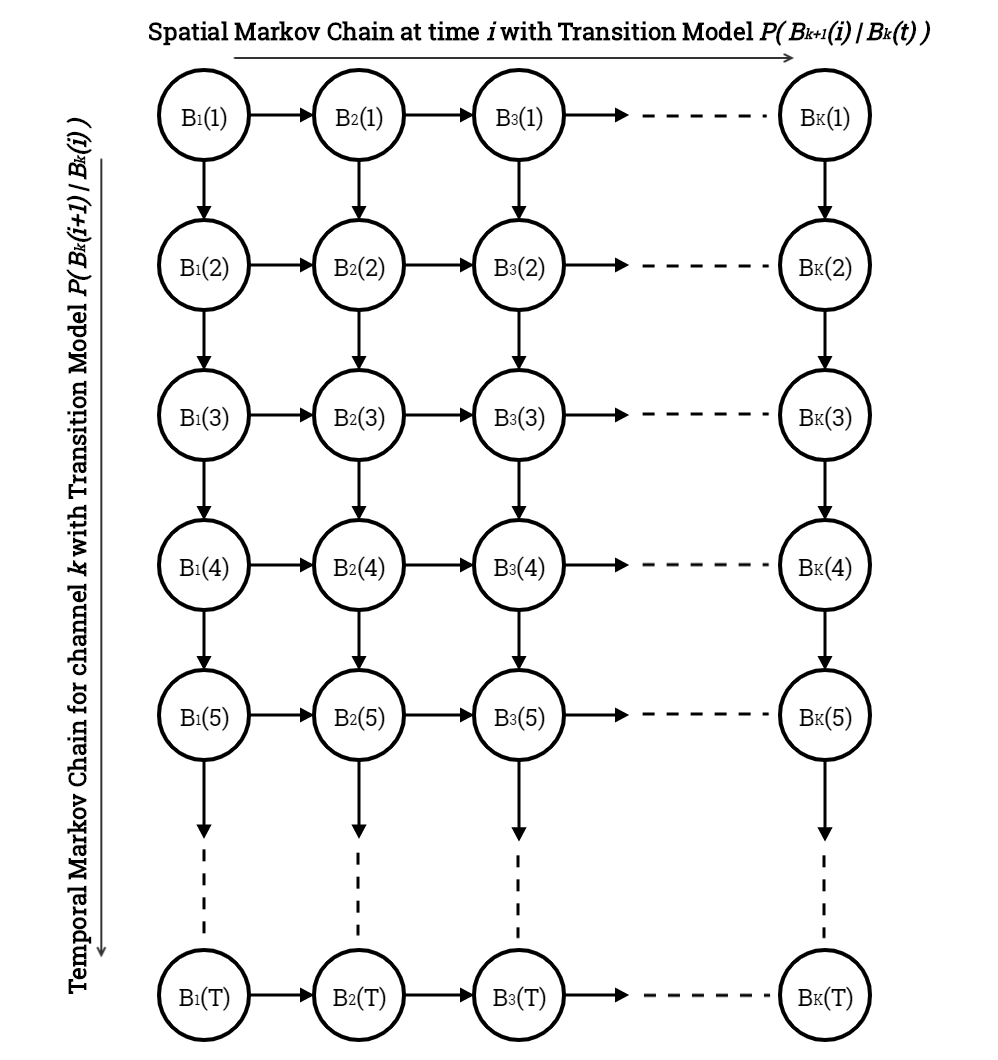
\includegraphics[scale=0.063]{minerva_occupancy_markov_chain.png}
    \caption{The correlation model across time and across frequencies underlying the occupancy behavior of incumbents in the network}
    \label{fig:1}
\end{figure}
\subsection{PU Spectrum Occupancy Model}
We now introduce the model of PU occupancy over time and across the frequency domain. We model each $X_k(i)$ as 
\begin{equation}\label{4}
    X_k(i)=\sqrt{P_{tx}}B_k(i)S_k(i),
\end{equation}
where $P_{tx}$ is the transmission power of the PUs, $S_k(i)$ is the transmitted symbol modelled as a constant amplitude signal, $|S_k(i)|=1$, i.i.d. over time and across frequency bands; \footnote{In the case where $S_k(i)$ does not have constant amplitude, we may approximate $H_{k}(i)S_{k}(i)$ as complex Gaussian with zero mean and variance $\sigma_H^2\mathbb E[|S_{k}(i)|^2]$, without any modification to the subsequent analysis.} $B_k(i)\in\{0,1\}$ is the binary spectrum occupancy variable, with $B_k(i)=1$ if the $k$th spectrum band is occupied by a PU at time $i$, and $B_k(i)=0$ otherwise. Therefore, the PU occupancy behavior in the entire wideband spectrum of interest at time $i$, discretized into narrow-band frequency components can be modeled as the vector 
\begin{equation}\label{5}
    \vec{B}(i)\ =\ [B_1(i),B_2(i),B_3(i),\cdots,B_K(i)]^T \in \{0,1\}^K.
\end{equation}
PUs join and leave the spectrum at random times. To capture this temporal correlation in the spectrum occupancy dynamics of PUs, we model the spectrum occupancy dynamics as a Markov process: given $\vec{B}(i)$, the spectrum occupancy state at time index $i$, $\vec{B}(i+1)$ is independent of the past, $\vec{B}(j),\ j < i$; $j, i \in \{1,2,3,\dots,T\}$, i.e. 
\begin{equation}\label{6}
    \begin{aligned}
        \mathbb{P}(\vec{B}(i+1)|\vec{B}(j),\ \forall j \leq i)\ =\ \mathbb{P}(\vec{B}(i+1)|\vec{B}(i)).
    \end{aligned}
\end{equation}
Additionally, when joining the spectrum pool, PUs occupy a number of adjacent spectrum bands, and may vary their spectrum needs depending on traffic demands, channel conditions, etc. To capture this behavior, we model $\vec{B}(i)$ as having Markovian correlation across the bands as, 
\begin{align}\label{7}
&         \mathbb{P}(\vec{B}(i+1)|\vec{B}(i))\\&=
\nonumber
         \mathbb{P}(B_{1}(i+1)|B_{1}(i))
         \prod_{k=2}^{K}\ \mathbb{P}(B_{k}(i+1)|B_{k}(i),B_{k-1}(i+1)).
\end{align}
That is, the spectrum occupancy at time $i+1$ in frequency band $k$, $B_{k}(i+1)$, depends on the  occupancy state of the adjacent spectrum band at the same time, $B_{k-1}(i+1)$, and that of the same spectrum band $k$ in the previous time index $i$, $B_{k}(i)$ as shown in Fig. \ref{fig:1}.
\subsection{Spectrum Sensing Model}
In order to detect the available spectrum holes, the SU performs spectrum sensing. However, owing to physical design limitations at the SU's spectrum sensor \cite{5990482}, not all channels in the discretized spectrum can be sensed at once. Therefore, due to limited sensing capabilities, the SU can sense only $\kappa$ out of $K$ spectrum bands at any given time, with $1\leq \kappa\leq K$. Let $\mathcal K_{i}\subseteq\{1,2,\dots,K\}$ with $|\mathcal K_i|\leq \kappa$ be the set of indices corresponding to the spectrum bands sensed by the SU at time $i$, which is part of our design.
Then, we define the observation vector
\begin{equation}\label{8}
    \vec{Y}(i)\ =\ [Y_k(i)]_{k\in\mathcal K_i},
\end{equation}
where $Y_k(i)$ is given by \eqref{3}.
The true states $\vec{B}(i)$ encapsulate the actual occupancy behavior of the PU and the measurements at the SU are noisy observations of these true states which are modeled to be the observed states of a Hidden Markov Model (HMM). Given the spectrum occupancy vector $\vec{B}(i)$ and the set of sensed spectrum bands $\mathcal K_i$, the probability density function of $\vec{Y}(i)$ is expressed as
\begin{equation}\label{9}
    f(\vec{Y}(i)|\vec{B}(i),\mathcal K_i)=\prod_{k\in\mathcal K_i}f(Y_k(i)|B_k(i)),
\end{equation}
owing to the independence of channels, noise, and transmitted symbols across frequency bands. Moreover, from \eqref{3} we find that
\begin{equation}\label{10}
 Y_k(i)|B_k(i)\sim \mathcal{CN}(0,\sigma_H^2P_{tx}B_k(i)+\sigma_V^2).
\end{equation}
\subsection{POMDP Agent Model}
In this section, we model the spectrum access scheme of the SU as a Partially Observable Markov Decision Process (POMDP) wherein the goal of the POMDP agent is to devise an optimal sensing and access policy in order to maximize its throughput while maintaining strict non-interference compliance with incumbent transmissions. In fact, the agent's limited sensing capabilities coupled with its noisy observations result in an increased level of uncertainty at the agent's end about the occupancy state of the spectrum under consideration and the exact effect of executing an action on the radio environment. The transition model of the underlying MDP as described by \eqref{7}, is denoted by $\mathbf{A}$ and is learned by the agent by interacting with the radio environment. The emission model is denoted by $\mathbf{M}$ and is given by \eqref{9}, with $f(Y_k(i)|B_k(i))$ given by \eqref{10}. 

We model the POMDP as a tuple $(\mathcal B,\mathcal{A},\mathcal{Y},\mathbf{P},\mathbf{M})$ where $\mathcal{B}\equiv\{0,1\}^K$ represents the state space of the underlying MDP with states $\vec{B}$ given by all possible realizations of the spectrum occupancy vector as described by \eqref{3}, $\mathcal{A}$ represents the action space of the agent, given by all $\left(\begin{array}{c}K\\\kappa\end{array}\right)$ possible combinations in which the $\kappa$ spectrum bands are chosen to be sensed out of $K$ at any given time; and $\mathcal{Y}$ represents the observation space of the agent based on the signal model outlined in the previous subsection. 
The state of the POMDP at time $i$ is given by the \emph{prior belief} $\beta_i$, which represents the probability distribution of the underlying MDP state $\vec{B}(i)$, given the information collected by the agent up to time $i$, but before collecting the new information in slot $i$. At the beginning of each time index $i$, given $\beta_i$, the agent selects $\kappa$ spectrum bands out of $K$ according to a policy $\pi(\beta_i)$, thus defining the sensing set $\mathcal K_i$, performs spectrum sensing  on these spectrum bands, observes $\vec{Y}(i)\in \mathcal{Y}$, and updates its \emph{posterior belief} $\hat{\beta}_i$ of the current spectrum occupancy $\vec{B}(i)$ as 
\begin{align}\label{11}
\hat\beta_i\ &=\ \mathbb{P}(\vec{B}(i)=\vec{B}'|\vec{Y}(i),\mathcal K_i, \beta_i)\\&=
\nonumber
\frac{\mathbb{P}(\vec{Y}(i)|\vec{B}',\mathcal{K}_i)\ \beta_i(\vec{B}')}{
\sum_{\vec{B}''\in\{0,1\}^K}\mathbb{P}(\vec{Y}(i)|\vec{B}'',\mathcal{K}_i)\ \beta_i(\vec{B}'')},
\end{align}
where $\mathbb{P}(\vec{Y}(i)|\mathcal{K}_i,\beta_{i-1})$ denotes the normalization constant and $\beta_{i-1}$ represents the belief of the agent prior to the observation $\vec{Y}(i)$, defined as a probability distribution over all possible states. 

Given the posterior belief $\hat{\beta}_i$, we employ a threshold based detection mechanism to determine whether a given channel is occupied ($\phi_k(\hat{\beta}_i) = 1$) or idle ($\phi_k(\hat{\beta}_i) = 0$). If a channel $k$ is deemed to be idle by this threshold based detection mechanism, the SU accesses it for the delivery of its network flows. On the other hand, if a channel $k$ is deemed to be occupied, the SU leaves it untouched. Furthermore, for utility evaluation, since relying on feedback from the radio environment will introduce unforeseen variables and additional dynamics into the problem, we use the state estimator detailed in Sec. \ref{III} to determine the reference occupancy metrics of the incumbents (the reference estimated state vector) $\hat{\vec{B}}$ based on the observations $\vec{Y}(i)$ obtained from the POMDP agent's sensing action, i.e. $\kappa_i$. Based on the number of \emph{truly idle} bands detected by the SU accounting for the throughput maximization aspect of the agent's end-goal and a penalty for \emph{missed detections} accounting for the incumbent non-interference constraint, the reward to the agent is modeled as
\begin{equation}\label{12}
    R(\hat{\vec{B}}(i), \hat{\beta}_i) = \sum_{k=1}^{K}(1 - \hat{B}_k(i))(1-\phi_k(\hat{\beta}_{i})) - \lambda \hat{B}_k(i)(1 - \phi_k(\hat{\beta}_i)),
\end{equation}
where $\lambda > 0$ represents the cost term penalizing the agent for missed detections, i.e. interference with the incumbent. After performing data transmission, the SU computes the prior belief for the next slot as
\begin{equation}\label{13}
    \beta_{i+1} = \mathbb{P}(\vec{B}(i+1) = \tilde{\vec{B}}|\mathcal{K}_{i+1}, \hat{\beta}_{i}).
\end{equation}
The optimization objective of the problem at hand can be written as
\begin{equation}\label{14}
    \pi^{*} = \argmin_{\mathcal{K}_{i} \in \mathcal{A}}\ \mathbb{E}\Big[\sum_{i = 0}^{\infty}\ \gamma^{i} R(\vec{B}(i), \mathcal{K}_{i})\ |\ \beta_0 = \beta\Big],
\end{equation}
where $0 < \gamma < 1$ is the discount factor and $\beta_0$ is the initial belief. The action policy $\pi$ of the agent maps the beliefs $\beta_i$ to actions $\mathcal{K}_i$ at time $i$ and is characterized by a value function
\begin{equation}\label{15}
V^{\pi}(\beta)\ =\ \mathbb{E}_{\pi}\ \Big[\sum_{i = 0}^{\infty}\ \gamma^{i} R(\vec{B}(i), \pi(\beta_{i}))\ |\ \beta_0 = \beta\Big],
\end{equation}
where $\pi(\beta_i)$ is the action taken by the agent at time $i$ under policy $\pi$. The optimal policy $\pi^*$ specifies the optimal action to take at the current time index assuming that the agent behaves optimally at future time indices as well. It is evident from equation \eqref{15} that we have an infinite-horizon discounted reward problem formulation and in order to solve for the optimal policy we need to solve the Bellman equation given by
\begin{equation}\label{16}
    V^*(\beta)=\max_{\mathcal{K}\in\mathcal{A}}\Big[\sum_{\vec{B}\in\mathcal{B}}R(\vec{B},\mathcal{K})\beta(\vec{B})+\gamma \sum_{\vec{Y}\in\mathcal{Y}}\mathbb{P}(\vec{Y}|\mathcal{K},\beta)V^*(\hat{\beta})\Big].
\end{equation}

Given the high dimensionality of the spectrum sensing and access problem, i.e. the number of states of the underlying MDP scales exponentially with the number of bands in the spectrum, solving equation \eqref{16} using Exact Value Iteration and Policy Iteration algorithms is computationally infeasible. Additionally, solving for the optimal policy from equation \eqref{16} requires prior knowledge about the underlying MDP's transition model. Therefore, in this paper we present a framework to estimate the transition model of the underlying MDP online, while utilizing this learned model to solve for the optimal policy by employing Randomized Point-Based Value Iteration techniques, namely, the PERSEUS algorithm \cite{DBLP:journals/corr/abs-1109-2145}.
\section{Approaches and Algorithms}\label{III}
\subsection{Occupancy Behavior Transition Model Estimation}
In real-world implementations of cognitive radio systems, the transition model of the occupancy behavior of the PUs is not known to the SUs in the network and needs to be learned over time. The learned model then needs to be fed back to the POMDP agent as a stride in a two-step iterative routine in order to solve for the optimal policy. The system can learn the model either before triggering or during the operation of the POMDP agent. Inherently, the approach constitutes solving a parameter estimation problem formulated as
\begin{equation}\label{17}
    \mathbf{A}^{*}\ =\ \argmax_{\mathbf{A}}\ \mathbb{P}([\vec{Y}(i)]_{i=1}^{\tau}|\mathbf{A}),
\end{equation}
which is a Maximum Likelihood Estimation (MLE) problem, where $\mathbf{A}$ is defined as $\mathbb{P}(\vec{B}(i+1)|\vec{B}(i))$ and $\tau$ refers to the learning period of the parameter estimator: this, as mentioned earlier, can be equal to the entire duration of the POMDP agent's interaction with the radio environment or can be a predefined parameter learning period before triggering the POMDP agent. In order to facilitate better readability, for the description of this parameter estimator, we denote $[\vec{Y}(i)]_{i=1}^{\tau}$ as $\mathbf{Y}$ and $[\vec{B}(i)]_{i=0}^{\tau}$ as $\mathbf{B}$. Re-framing \eqref{17} as an optimization of the log-likelihood, using the definition of marginal probability, and focusing on the joint instead of the conditional, we get,
\begin{equation}\label{18}
    \mathbf{A} = \argmax_{\mathbf{A}}\ \log\Big(\sum_{\mathbf{B}}\ \mathbb{P}(\mathbf{B}, \mathbf{Y}, \mathbf{A})\Big).
\end{equation}
In order to exploit the characteristics of the stated Markov model, we multiply and divide the operand of the logarithm by $\rho$ which from the equality constraint of Jensen's Inequality turns out to be $\mathbb{P}(\mathbf{B}|\mathbf{Y}, \hat{\mathbf{A}})$. The optimization problem in \eqref{18} is then restated as,
\begin{equation}\label{19}
    \begin{aligned}
        \mathbf{A} = \argmax_{\mathbf{A}}\ \sum_{\mathbf{B}}\ \mathbb{P}(\mathbf{B}|\mathbf{Y}, \hat{\mathbf{A}})\ \log(\mathbb{P}(\mathbf{B}, \mathbf{Y}, \mathbf{A})).
    \end{aligned}
\end{equation}
Applying the characteristics of the Markov model discussed in Sec. \ref{II}, we write \eqref{19} as
\begin{equation}\label{20}
    \begin{aligned}
        \mathbf{A}=\argmax_{\mathbf{A}}\sum_{\mathbf{B}}\mathbb{P}(\mathbf{B}|\mathbf{Y},\hat{\mathbf{A}})\sum_{L}\sum_{R}\sum_{i=1}^{\tau}\sum_{j=1}^{\tau}&\mathcal{I}\log(M_R(\vec{Y}(i)))\\
        &+\mathcal{J}\log(a_{LR}),
    \end{aligned}
\end{equation}
where $L,R \in \{0,1\}^K$ represent iterables for the occupancy state vectors,
\begin{equation}\label{21}
    \mathbf{M}_R(\vec{Y}(i)) = \mathbb{P}(\vec{Y}(i)|\vec{B}(i)=R),
\end{equation}
represents the emission model outlined in \eqref{9},
\begin{equation}\label{22}
    a_{LR} = \mathbb{P}(\vec{B}(i)=R|\vec{B}(i-1)=L, \hat{\mathbf{A}}),
\end{equation}
represents the unknown transition model which is the subject of this estimation, and $\mathcal{I}$ and $\mathcal{J}$ detailed below are indicator random variables introduced to bring in specificity into the estimation procedure.
\begin{equation}\label{23}
    \mathcal{I} = 
    \begin{cases}
        1, &\text{if}\ \vec{Y}(i)\ \text{and}\ \vec{B}(i)=R\\
        0, &\text{otherwise}
    \end{cases}
\end{equation}
\begin{equation}\label{24}
    \mathcal{J} = 
    \begin{cases}
        1, &\text{if}\ \vec{B}(i-1)=L\ \text{and}\ \vec{B}(i)=R\\
        0, &\text{otherwise}
    \end{cases}
\end{equation}
We impose a constraint on the transition probability in \eqref{22} as 
\begin{equation}\label{25}
    \sum_{R}\ a_{LR} = 1,    
\end{equation}
and formulate the Lagrangian as
\begin{equation}\label{26}
    \begin{aligned}
        \mathcal{L}=\Big\{\sum_{\mathbf{B}}\mathbb{P}(\mathbf{B}|\mathbf{Y},\hat{\mathbf{A}})\sum_{L}\sum_{R}\sum_{i=1}^{\tau}\sum_{j=1}^{\tau}&\mathcal{I}\log(\mathbf{M}_R(\vec{Y}(i)))\\
        &+\mathcal{J}\log(a_{LR})\Big\}\\
        +\sum_{L}\lambda_L(1-\sum_Ra_{LR}).
    \end{aligned}
\end{equation}
Solving for $a_{LR}$, we get,
\begin{equation}\label{27}
    a_{LR} = \frac{\sum_{i=1}^{\tau}\mathbb{P}(\mathbf{Y},\mathbf{A},\vec{B}(i)=R,\vec{B}(i-1)=L)}{\sum_{i=1}^{\tau}\mathbb{P}(\mathbf{Y},\mathbf{A},\vec{B}(i-1)=L)}.
\end{equation}
In order to further simplify \eqref{27} and bring it into an iterative algorithmic form, we introduce the forward and backward probabilities. We define the forward probability as
\begin{equation}\label{28}
    \begin{aligned}
        F(i,R) &= \mathbb{P}([\vec{Y}(t)]_{t=1}^{i},\vec{B}(i)=R)\\
        &= 
        \sum_{L}\mathbb{P}(\vec{B}(i)=R,\vec{Y}(i)|\vec{B}(i-1)=L)F(i-1,L),
    \end{aligned}
\end{equation}
and the backward probability as
\begin{equation}\label{29}
    \begin{aligned}
        D(i,L) &= \mathbb{P}([\vec{Y}(t)]_{t=i}^{\tau}|\vec{B}(i-1)=L)\\
        &= \sum_{R}\mathbb{P}(\vec{B}(i)=R,\vec{Y}(i)|\vec{B}(i-1)=L)D(i+1,R).
    \end{aligned}
\end{equation}
Using these definitions, \eqref{27} can be rewritten as,
\begin{equation}\label{30}
    a_{LR} = \frac{\sum_{i=1}^{\tau}F(i-1,L)\mathbf{M}_R(\vec{Y}(i))a_{LR}D(i+1,R)}{\sum_R\sum_{i=1}^{\tau}F(i-1,L)\mathbf{M}_R(\vec{Y}(i))a_{LR}D(i+1,R)}.
\end{equation}
\subsection{Occupancy Behavior State Estimation}
During the reward evaluation phase of the POMDP agent at time $i$, the observations made based on the sensing action $\mathcal{K}_i$ are employed at a state estimator to determine the occupancy state of the spectrum bands. Based on this estimated state vector, we formulate the false alarm and missed detection metrics which allow us to capture the throughput maximization and PU non-interference requirements essential for the operation of our POMDP agent. We formulate the state estimation problem as
\begin{equation}\label{31}
    \vec{B}(i)^* = \argmax_{\vec{B}}\ \mathbb{P}(\vec{B}|\vec{Y}(i)),
\end{equation}
which is a Maximum-A-Posteriori (MAP) estimation problem. This optimization problem can be restated in terms of the value functions as
\begin{equation}\label{32}
    W_{i,k}^{r} = \max_{\Tilde{\mathbf{B}}_{[t-1,k-1]}}\ \mathbb{P}(\Tilde{\mathbf{Y}}_{[t-1,k-1]},\Tilde{\mathbf{B}}_{[t-1,k-1]},Y_k(i),B_k(i)),
\end{equation}
where for the estimation of the occupancy in spectrum band $k$ at time $i$, 
\begin{equation}\label{33}
    \Tilde{\mathbf{Y}}_{[t-1,k-1]} \equiv \{\ [\vec{Y}_v(i)]_{v=1}^{k-1},\ [\vec{Y}_k(t)]_{t=1}^{t-1}\ \}
\end{equation}
denotes the set of all essential past observations which for readability purposes is denoted simply as $\Tilde{\mathbf{Y}}$ and
\begin{equation}\label{34}
    \Tilde{\mathbf{B}}_{[t-1,k-1]} \equiv \{\ [\vec{B}_v(i)]_{v=1}^{k-1},\ [\vec{B}_k(t)]_{t=1}^{t-1}\ \}
\end{equation}
denotes set of all essential past states which is henceforth simply referred to as $\Tilde{\textbf{B}}$ for readability. Applying the characteristics of the Markov model detailed in \eqref{7} to \eqref{32}, we get
\begin{equation}\label{35}
    \begin{aligned}
        W_{i,k}^{r} = \mathbf{M}_r(Y_k(i))\max_{\Tilde{\mathbf{B}}}\mathbb{P}(&B_k(i)=r|B_{k}(i-1)=m,\\
        &B_{k-1}(i)=n)\mathbb{P}(\Tilde{\mathbf{Y}},\Tilde{\mathbf{B}}),
    \end{aligned}
\end{equation}
which can be simplified further to show that,
\begin{equation}\label{36}
    \begin{aligned}
        W_{i,k}^{r} = \mathbf{M}_r(Y_k(i))\max_{m,n}\ a_{mnr}W_{i-1,k}^{m}W_{i,k-1}^{n},
    \end{aligned}
\end{equation}
where
\begin{equation}\label{37}
    a_{mnr} = \mathbb{P}(B_k(i)=r|B_{k}(i-1)=m,B_{k-1}(i)=n),
\end{equation}
which can be evaluated from the estimated transition model. Equation \eqref{36} corresponds to the forward recursion aspect of the double Markov chain Viterbi algorithm. Next, similar to the backtracking procedure in the one dimensional (single Markov chain) Viterbi algorithm, the Trellis diagram is traversed backwards to recover the most probable previous neighbours of $B_k(i)$. This is done recursively until the entire Trellis diagram has been traversed to yield the most probable state sequence, i.e. the Viterbi path. Mathematically, the backtracking step with respect to the neighbours of $B_k(i)$ is represented as
\begin{equation}\label{38}
    m^*, n^* = \argmax_{m,n}\ a_{mnr}W_{i-1,k}^{m}W_{i,k-1}^{n},
\end{equation}
where $m^*$ is the most probable state of channel $k$ in time index $i-1$ and $n^*$ is the most probable state of channel $k-1$ in time index $i$, given that channel $k$ in time index $i$ is in state $r$; $m, n, r \in \{0,1\}$.
\subsection{The PERSEUS Algorithm}
\begin{figure}
    \centering
    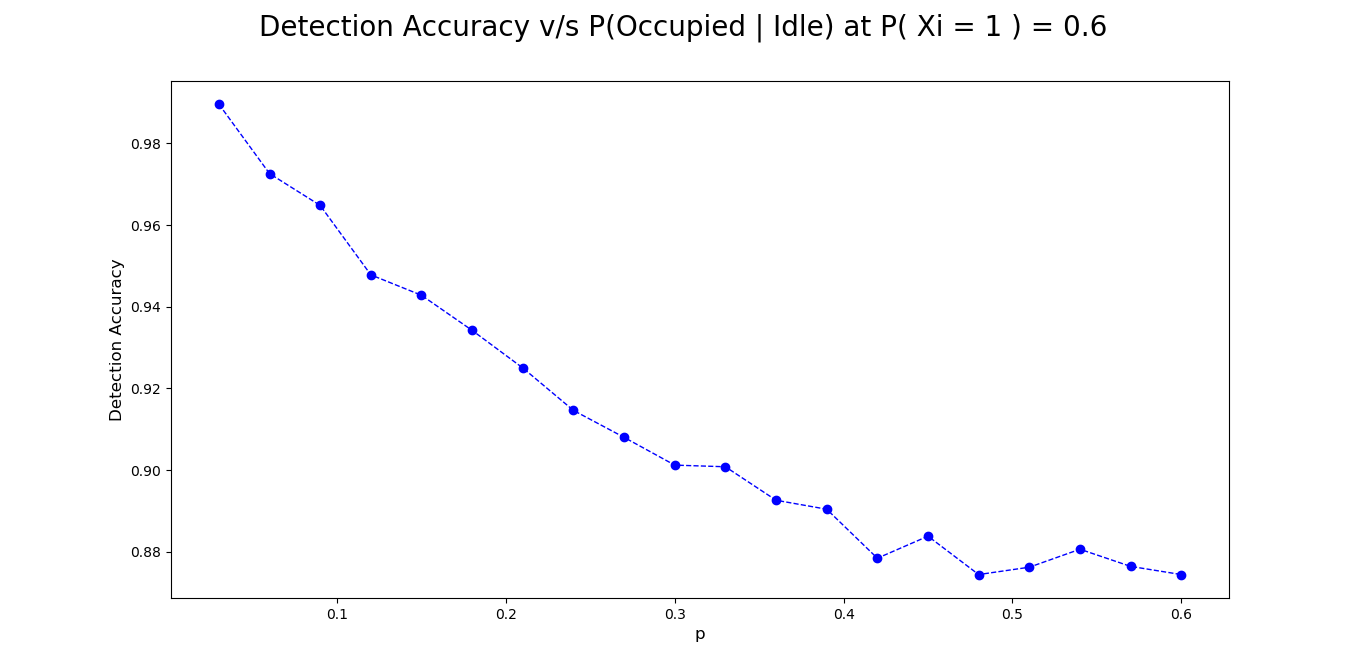
\includegraphics[scale=0.255]{DetectionAccuracy_v_p_test_3_final.png}
    \caption{The detection accuracy of the unconstrained Viterbi algorithm over varying values of $\mathbb{P}(\text{Occupied}|\text{Idle})$}
    \label{fig:2}
\end{figure}
\begin{figure}
    \centering
    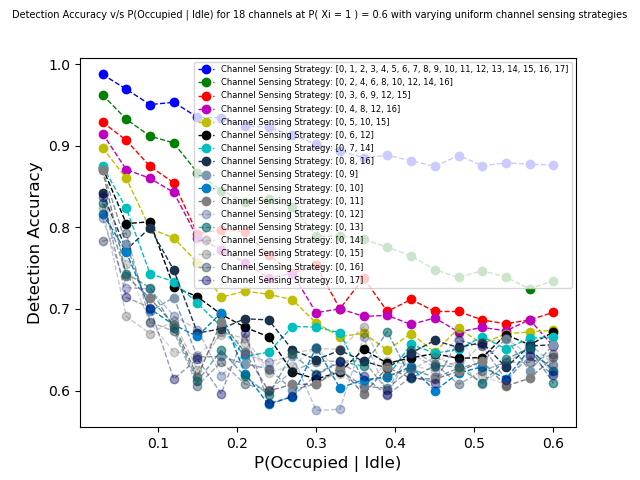
\includegraphics[scale=0.5]{Uniform_Channel_Sensing.png}
    \caption{The detection accuracies of the constrained Viterbi algorithm for different sensing strategies over varying values of$\mathbb{P}(\text{Occupied}|\text{Idle})$}
    \label{fig:3}
\end{figure}
\begin{figure}
    \centering
    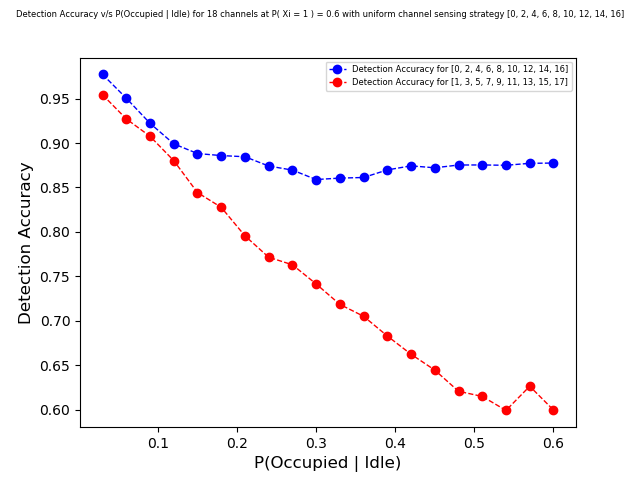
\includegraphics[scale=0.5]{Uniform_Channel_Sensing_1.png}
    \caption{The detection accuracies of the constrained Viterbi algorithm for sensed and un-sensed channels under a given channel sensing strategy}
    \label{fig:4}
\end{figure}
As discussed in Sec. \ref{II} of this article, solving the Bellman equation \eqref{16} for POMDPs with large state and action space using exact value iteration and policy iteration techniques \cite{Kaelbling:1998:PAP:1643275.1643301} is computationally infeasible \cite{DBLP:journals/corr/abs-1109-2145, Pineau:2003:PVI:1630659.1630806}. Hence, we resort to approximate value iteration techniques to ensure that the system scales well to a large number of bands in the spectrum of interest. For infinite-horizon POMDPs, $V^*$ in \eqref{16} can be approximated by a Piece-Wise Linear and Convex function (PWLC) \cite{Kaelbling:1998:PAP:1643275.1643301}. The core idea behind the PERSEUS algorithm is that the value function in time index $i$ can be parameterized by a set of hyperplanes $\{\vec{\alpha}_i^{u}\}$, $u = \{0,1,2,\dots,|V_i|\}$, each of which represents a region of the belief space for which it is the maximizing element. The backup step is defined as the process of determining the optimal hyperplane out of the set of available hyperplanes in time index $i$ as
\begin{equation}\label{39}
    \vec{\alpha}_{i}(\beta) = \argmax_{\vec{\alpha}_{i}^u} \beta \cdot \vec{\alpha}_{i}^u,
\end{equation}
which implies that,
\begin{equation}\label{40}
    \begin{split}
        V_i(\beta) &= \max_{\vec{\alpha}_{i}^u} \beta \cdot \vec{\alpha}_{i}^u,\\
        \pi_i(\beta) &= a(\vec{\alpha}_i^{u*}),
    \end{split}
\end{equation}
where $a(\vec{\alpha}_i^{u*})$ refers to the action corresponding to the optimal hyperplane. The PERSEUS algorithm constitutes an Exploration phase wherein the POMDP agent randomly interacts with the radio environment to collect a set of so-called reachable beliefs which are to be improved over numerous iterative backup stages. In each backup stage, the agent samples a belief $\beta$ uniformly at random from the set of unimproved points and performs a backup on this sampled belief point according to \eqref{39} to determine the optimal hyperplane $\vec{\alpha}$. Considering an arbitrary time index $i$, if $V_{i+1}(\beta) = \beta \cdot \vec{\alpha} \geq V_{i}(\beta)$, then the belief point $\beta$ is said to be improved along with any other belief points $\beta'$ in the unimproved set for which $V_{i+1}(\beta') = \beta' \cdot \vec{\alpha} \geq V_{i}(\beta')$. If $V_{i+1}(\beta) = \beta \cdot \vec{\alpha} < V_{i}(\beta)$, then a copy of the maximizing hyperplane for $V_i(\beta)$ is used for $V_{i+1}(\beta)$ and the belief point $\beta$ is then removed from the set of unimproved points. The backup stage continues until the set of unimproved points is empty and the agent performs a series of backup stages until there the number of policy changes between iterations is below a specified threshold $\eta$.

The belief update procedure outlined in \eqref{11} is an essential aspect of the PERSEUS algorithm which can turn into a performance bottleneck for large state spaces due to the inherent iteration over all possible states. In order to circumvent this problem, we fragment the spectrum into much smaller, independent sets of correlated channels and then run the PERSEUS algorithm on these fragments by leveraging multi-processing and multi-threading tools available at our disposal in software frameworks. Furthermore, we avoid iterating over all possible states and allow only those state transitions we deem to be the most probable - for example, we allow only those state transitions that involve a Hamming distance of up to 3 between the previous state vector and the current state vector in an 18 channel radio environment.
\section{Numerical Evaluation}\label{IV}
\begin{figure}
    \centering
    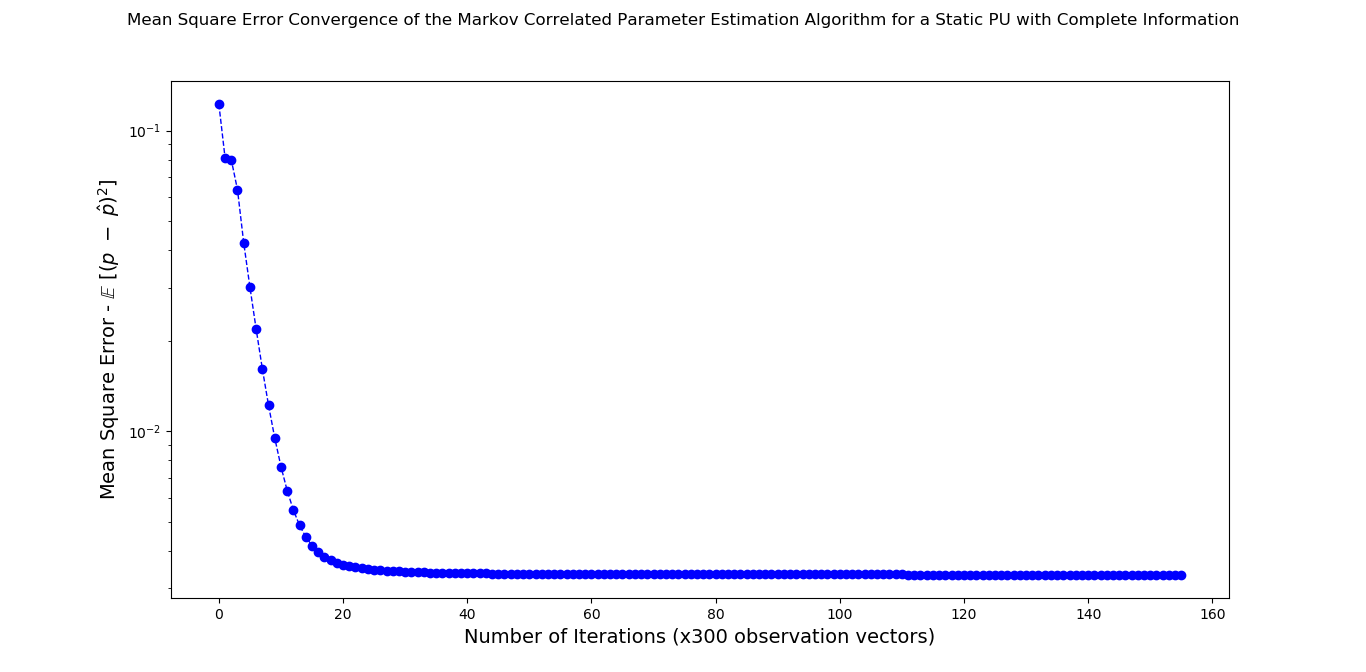
\includegraphics[scale=0.25]{Mean_Square_Plot_Log_Scale.png}
    \caption{The mean square error convergence plot of the parameter estimation algorithm\nm{Show x axis up to 40}}
    \label{fig:5}
\end{figure}
\begin{figure}
    \centering
    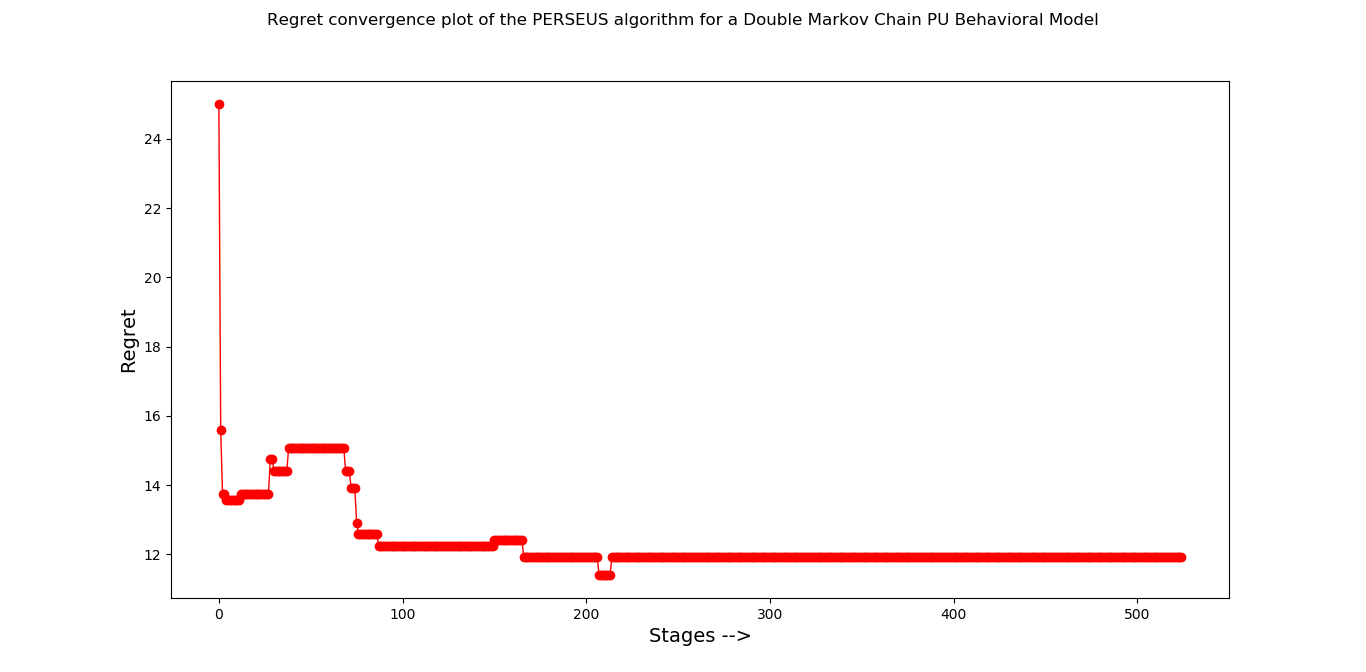
\includegraphics[scale=0.25]{Regret_Convergence_Plot_04112019.png}
    \caption{The regret convergence plot of the PERSEUS algorithm over several backup and wrapper stages}
    \label{fig:6}
\end{figure}
The given framework is simulated in Python for a system with 18 channels and a channel model constituting an SNR of 19dB when an incumbent occupies a specific channel. The same Markovian transition model, emission model, and steady-state model is employed across both the chain across time and the chain across frequencies. The plot depicted in Fig. \ref{fig:2} illustrates the detection accuracy of the Viterbi algorithm wherein the SU makes observations of all the channels in the radio environment and estimates the occupancy states of these channels over varying values of $\mathbb{P}(\text{Occupied}|\text{Idle})$, i.e., as the channels transition toward independence. We note that the detection accuracy of the state estimator degrades as the channels transition toward independence, which is as surmised, because the Viterbi algorithm's structure begins to crumble if the Markovian correlation ceases to exist among cells in the grid, where a cell corresponds to the state of a certain channel at a given time index.

Fig. \ref{fig:3} illustrates the detection accuracies of the Viterbi algorithm wherein the SU makes observations of only the channels in the given channel sensing strategy and estimates the occupancy states of both the sensed and the un-sensed channels over varying values of $\mathbb{P}(\text{Occupied}|\text{Idle})$. In Fig. \ref{fig:4}, the plot depicted shows the detection accuracies of the estimation of sensed and un-sensed channels for the constrained Viterbi algorithm in which the SU only senses channels whose indices correspond to the multiples of 2 and uses these channels to estimate the occupancy behavior of the incumbents across all 18 channels over varying values of $p = \mathbb{P}(\text{Occupied}|\text{Idle})$. In both these plots, we observe that, as anticipated, the detection accuracy of the state estimator deteriorates as the amount of information available for estimation reduces. 

The plot depicted in Fig. \ref{fig:5} shows the Mean Square Error convergence of the Parameter Estimation algorithm while determining the transition model of the MDP underlying the problem under consideration. Starting with an initial estimate of 0.0, the EM algorithm detailed in Sec. \ref{III} converges to the true transition model  with an error of $\epsilon \leq 10^{-8}$ over numerous iterations, each iteration corresponding to an averaging operation of 300 observation vectors. Here, we observe the mean square error given by $\mathbb{E}[(p - \hat{p})^{2}]$ iteratively reduces as it goes through the E-step which finds the distribution for the parameters in the current time-step, given the previous estimate and the M-step which determines the maximum likelihood estimate of the parameters, given the distribution obtained in the E-step. It has been theoretically shown to converge, i.e., each iteration either improves the true likelihood or leaves it unchanged \cite{Neal1998}. Since the EM algorithm is susceptible to premature convergence to local optima and saddle points, we mitigate this by averaging the procedure over several cycles.
\begin{figure}
\centering
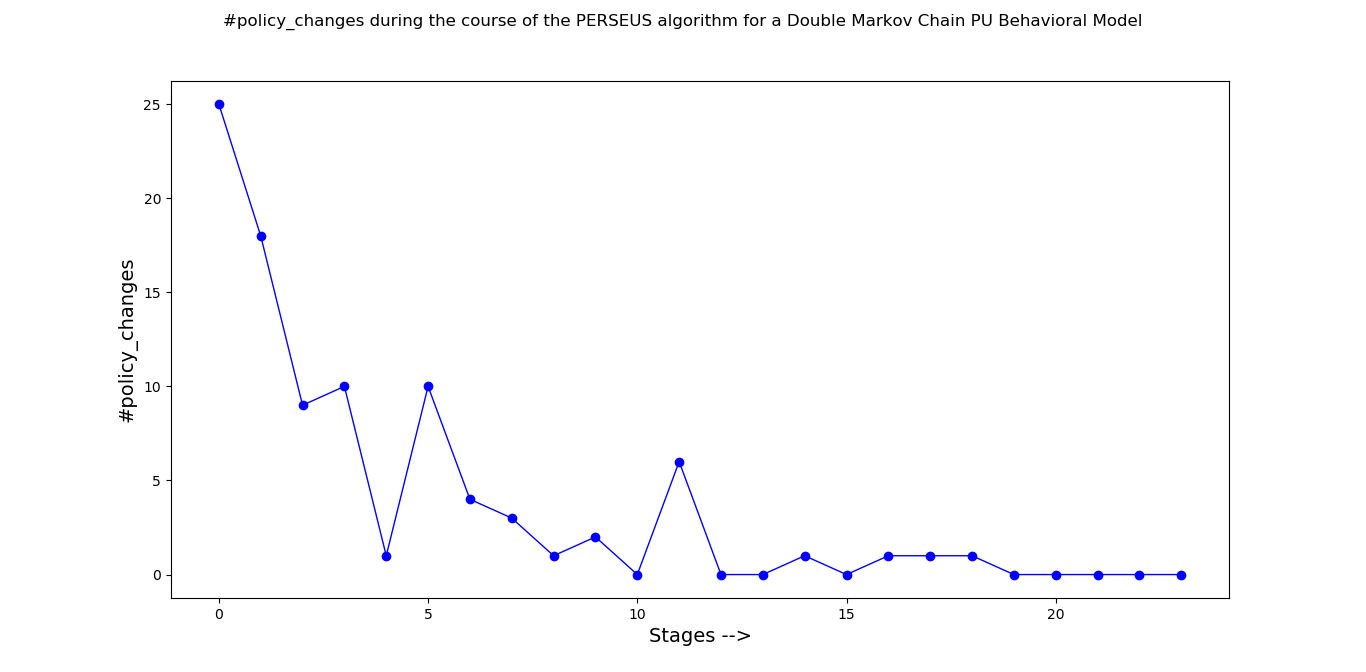
\includegraphics[scale=0.25]{Policy_Changes_Plot_04112019.png}
\caption{The number of policy changes involved in the PERSEUS algorithm as it transitions toward convergence over numerous backup and wrapper stages}
\label{fig:7}
\end{figure}

Fig. \ref{fig:6} illustrates the Regret Convergence plot of the PERSEUS algorithm over several backup and wrapper stages wherein the regret metric corresponds to the difference in utility between the PERSEUS algorithm at a certain stage and an Oracle which has complete information with respect to the occupancy behavior of the incumbents in the radio environment. Furthermore, the algorithm involves an online estimation of the transition model of the underlying MDP and a random exploration strategy to gather the initial set of reachable beliefs. Fig. \ref{fig:7} depicts the number of policy changes involved in each individual stage of the PERSEUS algorithm as it moves toward convergence. The termination condition for the PERSEUS algorithm is that the number of policy changes over several consecutive backup stages should be zero, i.e., $\eta = 0$. These plots, similar to the \textit{Reward v/s Time} and $\Delta \pi$ \textit{v/s time} plots in \cite{DBLP:journals/corr/abs-1109-2145}, serve as a measure of convergence for our fragmented PERSEUS algorithm with simplified belief updates, and an online transition model estimation.
\section{Conclusion}\label{V}
In this paper, we formulate the optimal spectrum sensing and access problem in an AWGN observation model with multiple licensed users and a cognitive radio node restricted in terms of its sensing capabilities, as a partially observable stochastic game. In a radio environment wherein the occupancy behavior of the incumbents is correlated across time and frequencies, we present a consolidated framework that employs the Expectation-Maximization algorithm to estimate the transition model of this occupancy behavior and leverage a fragmented PERSEUS algorithm with belief update heuristics to simultaneously solve for the optimal spectrum sensing and access policy. Through system simulations, we show that our framework out-performs the existing correlation-coefficient based state-of-the-art; surpasses Neyman-Pearson based occupancy detection schemes that fail to exploit the correlation across time and frequencies; and matches the performance of standard MAP-estimators which possess the transition model statistics as an apriori.
\bibliographystyle{IEEEtran}
\bibliography{ref}
\end{document}